\documentclass[12pt]{article}
\usepackage{indentfirst}
\usepackage{graphicx}
\usepackage{textcomp}
\usepackage{siunitx}
\usepackage{subcaption}
\usepackage{amsmath}
\usepackage{setspace}
\usepackage{url}
\usepackage[a4paper,margin=2.54cm]{geometry}

\title{Computer Science I \\Project 1: Animation}
\author{TAERAKUL Janat, \#19B60096}
\date{November 9, 2019}
\renewcommand{\UrlFont}{\small\tt}

\begin{document}

% \onehalfspacing
% \doublespacing

\maketitle

\section{Instruction}\label{sec:instr}

	This program is a python program. It takes a number as an input and shows the number on a sliding $10 \times 28$ pixels display. The display consists of numbers 0 and 1, which denote black and white pixels. Another function of this program is displaying first 100 digits of Pi ($\pi$). 

	To run this program, open terminal and go to the directory that contain \texttt{anime.py} file, then run \texttt{\$ python anime.py}.

	After the program is run, it will ask its user to enter a number or "pi" as shown in figure (\ref{fig:runProg}). If the user enter a number, the program will show that number moving right to left until the end of that number as figure (\ref{fig:runningProg}). If the user enter "pi", the program will shows the first 100 digits of Pi ($\pi$). In case the user enter something other than numbers and dot, the program will ignore that character and skip to the next one.

	\begin{figure}[ht]
		\centering
		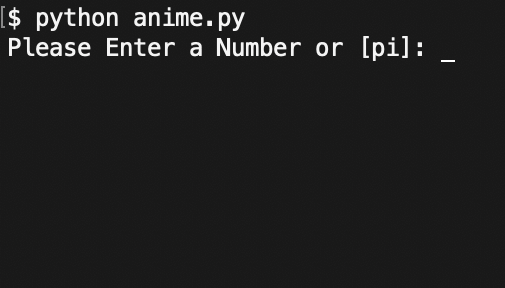
\includegraphics[height=3.5cm]{runProg.png}
		\caption{The program ask user to input a number.}
		\label{fig:runProg}
	\end{figure}	

	\begin{figure}[ht]
		\centering
		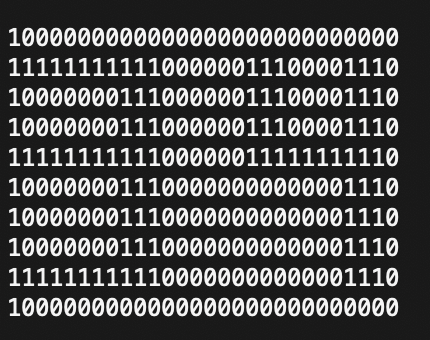
\includegraphics[height=4.5cm]{runningProg.png}
		\caption{The program showing the number inputed by user.}
		\label{fig:runningProg}
	\end{figure}

\section{How the Program Works}\label{sec:how}

	To do this project, I did research on how to define functions in python3. This program consists of several variables and functions which are explained as following.

	\subsection{Global Variables}

		\begin{enumerate}
			\item \texttt{img} - An array of 10 integers. Used as display of the program.
			\item \texttt{num} - A 2D array with 10 arrays of 10 integers. Used as templates for number 0-9.
			\item \texttt{dot} - An array of 10 integers. Used as template of a dot.
			\item \texttt{pi} - A string of first 100 digits of Pi ($\pi$)
		\end{enumerate}

	\subsection{Function}

		\begin{enumerate}
			\item \textbf{tenPow(n)} - Input an integer $n$ into this function,it returns $10^n$ back. 

			The variable $ans$ initially has value of $1$. The function has a loop for $n$ times, each time it multiply $ans$ by $10$ and return $ans$ when the loop ends.
				\begin{verbatim}
					def tenPow(n):
					  ans = 1
					  for i in range(n):
					    ans *= 10
					  return ans
				\end{verbatim}

			\item \textbf{mod(a, b)} - Input integer $a$ and $b$ into this function, it returns the remainder from dividing $a$ by $b$. I need modulo function to find the last digit of a number (Ex. $1324\ mod\ 10 = 4$). 

			The function can be implemented by subtracting $(a//b)*b$ from a. Since // is integer division, $(a//b)*b$ gives value of the most multiple of $b$ that less than or equal to $a$.
				\begin{verbatim}
					def mod(a, b):
					  return a - ((a//b) * b)
				\end{verbatim}

			\item \textbf{kthDigit(x, k)} - Input integer $x$ and $k$ into this function, it returns the $k^{th}$ digit from the last of $x$. 

			The function uses $mod 10$ to find the last digit of $x//10^{k-1}$, which is $k^{th}$, $(k+1)^{th}$, $...$ digits of $x$. (Example. $1234567//10^{3-1} = 12345$ and $12345\ mod\ 10 = 5$ which is the $3^{rd}$ digit of x)
				\begin{verbatim}
					def kthDigit(x, k):
					  return mod(x // tenPow(k-1), 10)
				\end{verbatim}

			\item \textbf{printImg()} - This function prints the value in variable $img$ and call function \texttt{time.sleep(0.1)} to pause the program for 0.1 second.
				\begin{verbatim}
					def printImg():
					  for line in img:
					    print(line)
					  print()
					  time.sleep(0.1)
				\end{verbatim}

			\item \textbf{showDigit(x)} - Input a number $x$ (0-9) into this function, it push the template in variable $num$ of the number $x$ into the display or the variable $img$.

			The function consists of two nested loops. The outer loop repeats 16 times as $k = 16, 15, ... ,2 , 1$. The inner loop repeats 10 times as $i = 0, 1, ..., 8, 9$, each time it push the \underline{$k^{th}$ digit of $i^{th}$ integer in the template of number $x$} into the \underline{$i^{th}$ integer of variable $img$}. 

			To shift all digits of $img[i]$ to the left, the function multiplies $img[i]$ by 10. Then add the $k^{th}$ digit of each integer in the template of number $x$ by using function \texttt{kthDigit()}. Now, $img[i]$ has 29 digits, which has to be changed to 28 digits. So, the function subtracts $10^{28}$ from $img[i]$. Lastly, if $img[i]$ does not have the $28^{th}$ digit from the last then the function adds $10^{27}$ to $img[i]$. 
				\begin{verbatim}
					def showDigit(x):
					  for k in range(16, 0, -1):
					    for i in range(10):
					      img[i] *= 10
					      img[i] += kthDigit(num[x][i], k)
					      img[i] -= tenPow(28)
					      img[i] += (1 - kthDigit(img[i],28)) * tenPow(27)
					    printImg()
				\end{verbatim}

			\item \textbf{showDot()} - This function push the template of a dot in the variable $dot$ into the display or the variable $img$ uy using the same method as function \texttt{addDigit()}.
				\begin{verbatim}
					def showDot():
					  for k in range(10, 0, -1):
					    for i in range(10):
					      img[i] *= 10
					      img[i] += kthDigit(dot[i], k)
					      img[i] -= tenPow(28)
					      img[i] += (1 - kthDigit(img[i],28)) * tenPow(27)
					    printImg()
				\end{verbatim}

			\item \textbf{showBlank()} - This function add 28 columns of zero into the display or the variable $img$ uy using the same method as function \texttt{addDigit()} and function \texttt{addDot()}.
				\begin{verbatim}
					def showBlank():
					  for k in range(28):
					    for i in range(10):
					      img[i] *= 10
					      img[i] -= tenPow(28)
					      img[i] += (1 - kthDigit(img[i],28)) * tenPow(27)
					    printImg()
				\end{verbatim}

			\item \textbf{show(ch)} - Input a character into this function, it decides to call a function between function \texttt{addDigit()} and function \texttt{addDot()}. If the input is a number, it calls function \texttt{addDigit()} and pass the input into the function. If the input is a dot, function \texttt{addDot()}. The function will ignore other types of input.
				\begin{verbatim}
					def show(ch):
					  if ch == '.':
					    showDot()
					  elif ch >= 48 and ch <= 57:
					    showDigit(ch - 48)
				\end{verbatim}

			\item \textbf{showNum(str)} - Input a string of a number into this function, it decodes the string to  a list of characters and pass each character into function \texttt{show()}. After it shows all character, it fills the display (variable $img$) with zeros.
				\begin{verbatim}
					def printNum(s):
					  ch = s.encode("ascii")
					  for digit in ch:
					    show(digit)
					  showBlank()
				\end{verbatim}
		\end{enumerate}

	\subsection{Main Program}
	When the program is run, the process starts from asking for input string from user. If the input string match "PI", "Pi", "pI", or "pi", the program sets value of input variable to pi (string of "3.14159..."). Then, the program passes the input into function \texttt{printNum()}
	\begin{verbatim}
		inp = input("Please Enter a Number or [pi]: ")
		if inp == 'PI' or inp == 'pi' or inp == 'Pi' or inp == 'pI':
		  inp = pi
		printNum(inp)
	\end{verbatim}

\end{document}